In this section we present the results from our evaluation of the two proposed algorithms.

\subsection{Client-side Speculation}
\Cref{fig:client-side-acceptance-rates} shows the throughput of various speculative models with different acceptance rates for the client-side algorithm {\it on a subset of the BFCL prompts}. 
We show these results on an easier to predict subset of tools, so that we can observe the behavior for values $\alpha > 0.8$ to validate \Cref{eq:client-alg-speedup}. In the later experiments we observed $\alpha \approx 0.8$ for xLAM-2-8B.
Results are shown for runs with an average tool latency of 1.5 seconds, but the trends are similar for other tool latency amounts.
Point annotations denote how many tool calls are speculated by the speculative model each turn ($\lambda$ in Algorithm~\ref{alg:spec-tool-cache})(e.g. $1\times$, $3\times$, ...).

\begin{figure}[h]
    \centering
    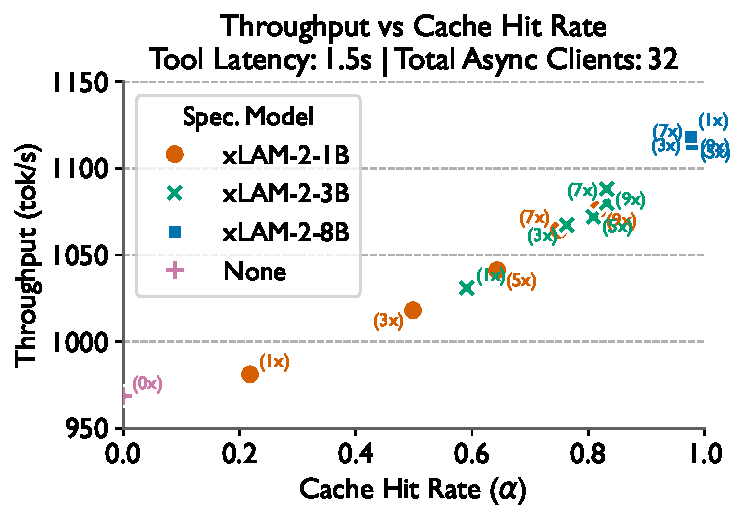
\includegraphics[width=\linewidth]{figs/acceptance_rates_tool_latency_1p5s}
    \caption{Throughput improvement for various speculative models and their cache hit respective tool cache hit rates. Points are annotated with the number of speculations per generation. We see a clear trend in improved throughput as the tool prediction rate increases. \label{fig:client-side-acceptance-rates}}
\end{figure}

We see that the trends from our performance model hold (see \Cref{sec:client-side-analysis}) hold; as speculation rate increases, we see an increase in inference throughput.
The 8B model yields much better accuracy in tool prediction than the smaller models, however, we see that the accuracy of the smaller models can also be improved by increasing the number of samples.
xLAM-2-1B achieves nearly 60\% higher hit rate with $9\times$ samples versus $1\times$ samples.
This flexibility is important as we may desire to run smaller speculative models due to memory constraints; taking more samples with a smaller model can get close to the performance of a larger speculative model.

\begin{figure}[ht]
    \centering
    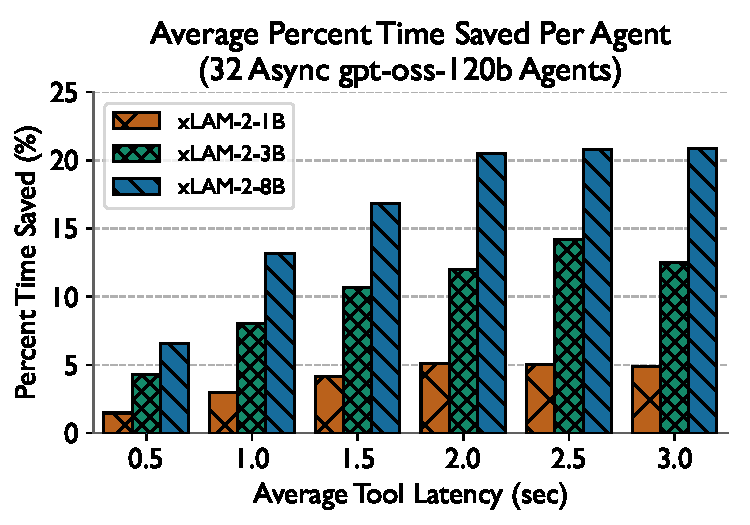
\includegraphics[width=0.92\linewidth]{figs/time-saved_32_clients_1_num_spec}
    \caption{Average percent time saved across runs with various speculative models and average tool latencies. Results are shown for $1\times$ speculation per generation. We see that client side speculation can lead to between 6-21\% end-to-end time saving per agent when average tool latencies are 0.5 to 3 seconds. \label{fig:client-side-time-saved}}
\end{figure}


\Cref{fig:client-side-time-saved} shows the average percent time saved for each agent being run using the client side speculative algorithm. 
Even for shorter tools, around 0.5 seconds in duration, we still observe noticeable improvements with up to 6\% of total time saved by speculating the tools.
Results improve as the average tool time approaches gpt-oss-120b's average generation time; when tools average around 2.0-2.5 seconds we see the biggest gains with up to 21\% saved. 
The percent time saved slowly decrease as tools dominate the runtime and speculation only provides minor savings for long lasting tools.
This behavior is further evidence to the performance models in \Cref{sec:client-side-analysis} where we observe that tool calls around the generation time of the main model lead to the highest speedups.

\begin{observationbox}{Client-side Speculation Benefits}
An agentic framework, without any additional changes to the inference engine or API, can achieve 6-21\% time saved by speculating tools ahead of time. Savings vary depending on the ratio of model generation time and average tool call duration.
\end{observationbox}

\begin{figure}[h]
    \centering
    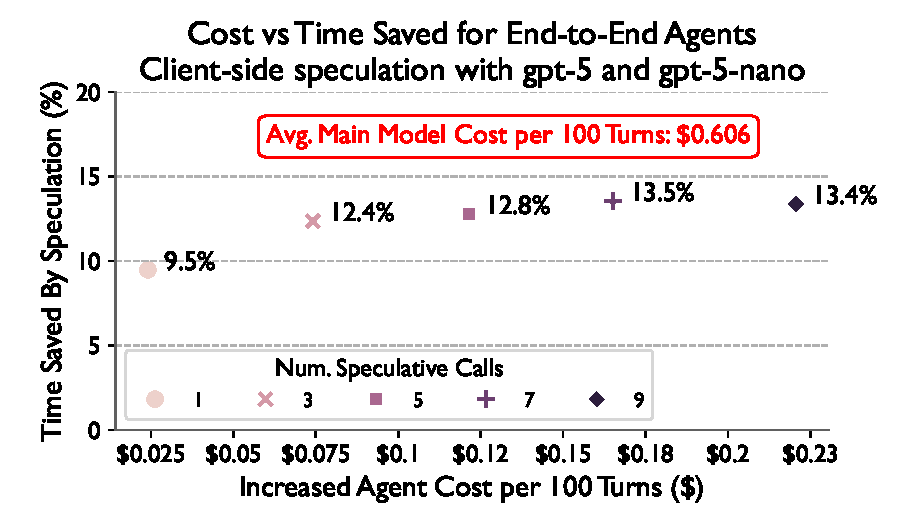
\includegraphics[width=\linewidth]{figs/results-cost-spec-client}
    \caption{The increased cost for running client-side speculation with gpt-5-nano alongside a gpt-5 agent. Costs are shown for 100 agent turns. For only a 4\% price increase, agents can save nearly 10\% time.\label{fig:spec-cost}}
\end{figure}

We can also run the client-side speculation algorithm for commercial models where we only have API access.
\Cref{fig:spec-cost} shows the percent time saved by using speculation versus the added cost of doing that speculation.
The results are presented for a single agent ``turn", or one API then tool call pair.
We see that with one speculation we can get nearly 10\% time savings with only an extra API call that is an order of magnitude cheaper than the main API call.
Running nine speculations increases the time saved marginally, but is around 25-30\% of the cost of the main generation.

\subsection{Engine-side Speculation}

\Cref{fig:result-engine-side} shows the percent time saved for the engine-side algorithm.
We additionally show the times for average tool latencies in $\{0.1, 0.2, 0.3, 0.4, 0.5\}$ to highlight the regime where engine-side speculation helps most.
vLLM's speculative decoding infrastructure, what we build our implementation on top of, is currently in an experimental development phase~\cite{noauthor_speculative_nodate_v2} and we found high overheads for its spec-dec implementation when the batch size is greater than 1. 
For this reason we present our engine-side results with only one asynchronous agent.
Note that when there is only one asynchronous agent we see much lower generation latency from vLLM due to the request scheduler and smaller batch. Our observations align with findings in other works~\cite{singhania_llm_2025}. This leads to less potential gains as there is less generation time to overlap tool calls with, so we see lower percent time saved than in \Cref{fig:client-side-time-saved}.

\begin{figure}[h]
    \centering
    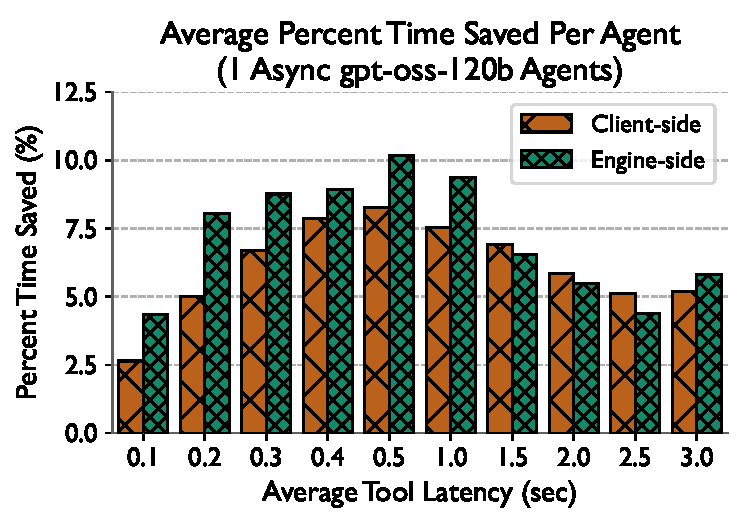
\includegraphics[width=\linewidth]{figs/time-saved_1_clients_1_num_spec_by-alg}
    \caption{Average percent time saved comparison between client-side and engine-side algorithms for various average tool latencies. Results shown for one async client and xLAM-2-8B for speculation. When tools finish before the main model is done reasoning, we can achieve 2-3\% better time savings than the client-side approach.\label{fig:result-engine-side}}
\end{figure}

\begin{observationbox}{Engine-side Speculation Benefits}
Posting speculated tool outputs to an inference server to keep sequences resident when tool outputs are available a priori can lead to an additional 2-3\% time saved from the client's perspective.
The best benefits occur where tools latencies are less than the main model $\mathcal{M}$'s reasoning time.
This is ideal as many common agent tools fall in the 0-1 second range (e.g. \texttt{ls}, web search, read file, ...).
\end{observationbox}

We see 2-3\% increased time savings in the engine-side algorithm compared to the client-side algorithm. This is on top of the already high savings from the client-side speculation.
We see the best results where tool calls are between 0 and 1 second as these finish and are posted to the inference server before the reasoning phase is done.
Longer tool calls do not see any benefit over client-side speculation, since their results are not posted to the inference server before decoding is ready.

